%!TEX root = main.tex

\chapter{Sampling, waveshaping, and non-linearity}
\label{Waveshaping}

\begin{center}
\begin{figure}[h!]
\tikzset{concept/.append style={fill={none}}}
\begin{tikzpicture}
  \path[mindmap,concept color=black,text=black]
    node[concept] {Sampling}
    [clockwise from=0]
    child[concept color=red!50!black] {node[concept] (rec) {recording} }
    child[concept color=green!80!black] {node[concept] (pla) {playback} }
    %   [clockwise from=90]
    %   child { node[concept] {algorithms} }
    %   child { node[concept] {data structures} }
    %   child { node[concept] {pro\-gramming languages} }
    %   child { node[concept] {software engineer\-ing} }
    % }
    child[concept color=blue] { node[concept] (ram) {in RAM vs. from Disk}[clockwise from=-30]}
    child[concept color=red] { node[concept] (gra) {granular} }
    child[concept color=orange] { node[concept] {Waveshaping and Distortion} };

\begin{pgfonlayer}{background}
	% \draw [draw=green,fill=black, decorate,decoration=circle connection bar]
    \draw [circle connection bar]
    % \path (rec) to[circle connection bar] (pla)
      (rec) edge (pla)
      (gra) edge (pla)
      (ram) edge (pla)
      ;
  \end{pgfonlayer}

\end{tikzpicture}
\caption{Lecture Contents}
\end{figure}
\end{center}

% \section{Notizen}

% Waveshaping generell.

% Evt. Subtraktiver Synth am ende.

% Zusammenhang waveshaping, distortion. lookup table, sampling, wavescanning.

% Waveshaping = modulation \cite[p.~257]{farnell_designing_2010}

% chebyshev

% \glqq{}intermod. distortion \grqq{} , vgl. miller puckette, \\
% http://msp.ucsd.edu/techniques/latest/book-html/node78.html

% middle term! ( (a+b)**2 = a**2 +2ab +b**2 )




% beispiele:
% sinus
% vllt:\\
% dyn. non-linear functions




% \section{Uebersicht}
% Zunächst: Sampling, dann lineare transfer function.

% \begin{enumerate}
% 	\item übersicht: fragen wies geht, wie ist es mit Max/MSP?
% 	\item HÜ ankündigen
% 	\item neue abstraction: z-1
% 	\item Raetsel
% 	\item Wo letztes mal stehngeblieben? Poly syth fertig?
% 	\item linearität erklären. Nun Nichtlinearität.
% 	\item wavetable/lookup wiederholung
% 	\item Lookup als waveshaping/distortion
% 	\item waveshaping durch processing vs. durch lookuptable
% 	\item durchrechnen
% 	\item chebyshev
% 	\item Sampling (Ram nicht Ram)
% 	\item send and receive von GUI f. Hausübung
% \end{enumerate}

\section{Waveshaping}


 \link{https://colab.research.google.com/github/hrtlacek/dspCourse/blob/master/notebooks/01\_sampling\_non-lin.ipynb}{Notebook for this Section}
\link{https://www.shadertoy.com/view/ws3fD4}{Shader for this Section}


Wikipedia quote, page ``waveshaper'':\\
\glqq{}The mathematics of non-linear operations on audio signals is difficult, and not well understood.\grqq{}
Waveshaping means distortion. It adds overtones, take a look at figure ~\ref{fig:waveshapedSIne}.


\begin{figure}[h!]
	\centering
	\includegraphics[width=11cm]{waveShapedSine.png}
	\caption[Wave shaped sine oscillator]
	{A sine wave has been generated and waveshaping was applied to add overtones.}
	\label{fig:waveshapedSIne}
\end{figure}


\begin{figure}[h!]
	\centering
	\includegraphics[width=11cm]{tanhTime.png}
	\caption[Distorted sine, time domain]
	{The same as the spectrogram above, but in the time domain. We can see the input sine wave and the slightly distorted output. It may look like just the amplitude has changed, but the sine's actual \textit{shape} has changed slightly}
	\label{fig:tanhTimeDom}
\end{figure}

\subsection{The simplest case: a linear Transfer function. } % (fold)
\label{sub:linearTrans}
See \ref{fig:linfunct}. A linear transfer function is used as a lookup table for a sinosoidal input.

\newpage

\begin{figure}[h]
	\begin{center}
		\includegraphics[scale = 1]{img/waveShapingVisual.png}
		\caption{Linear Transfer function}
		\label{fig:linfunct}
	\end{center}
\end{figure}
A transfer function in the sense of a waveshaper (a ``transfer function'' might also mean frequency response in other contexts) is a simple look-up function. \
Waveshaping means to use an input wave to \textit{look up} values in a table or function. A linear transfer function, let's call it $l$, can result in no change, for example, it might return $l(x)=x$. \
This means, that whatever value we pass in, we get the same value out.\
Other linear transfer functions might \textit{only} change the amplitude. For example $f(x)=x \cdot \frac{1}{2}$. That doesn't seem very interesting. But it might explain the term ``linear''. A transfer function is linear if it looks like a line if we plot it. Look at figure \ref{fig:linears}.

\begin{figure}[h!]
	\centering
	\includegraphics[width=15cm]{linearFunctions.png}
	\caption[Linear Transfer functions]
	{A couple of linear transfer functions and their corresponding effects demonstrated using a sine wave. From left to right: multiplication by 0.5, so attenuation by about 6dB, inversion, and the ``do-nothing''-function.}
	\label{fig:linears}
\end{figure}


Non-liner transfer functions behave differently. They map their input to other values, such as $f(x) = x^2$. And if we plot then, they don't look like a line.  You can also look at figure \ref{fig:farnellWaveShaping} in order to understand what's happening. We again see a linear transfer function but also a non linear one.
\begin{figure}[H]
	\centering
	\includegraphics[width=13cm]{waveshapingVizFarnell.png}
	\caption[farnell wave shaping visualization]
	{A waveshaping visualization taken from \cite{farnell_designing_2010}}
	\label{fig:farnellWaveShaping}
\end{figure}

But let's get back to our square function, since it's simpler and we will find some surprising results when analyzing it. Let's first simply plot it too.


\begin{figure}[H]
	\begin{center}
		\includegraphics[width = 14cm]{img/squareFunction.png}
		\caption{The function $f(x)=x^2$}
		\label{fig:square}
	\end{center}
\end{figure}

% subsection subsection_name (end)

\video{
What does applying a curve to every pixel of a video or image do? Is this even something people do? Of course! Think of contrast curves, below is an example from photoshop. Beware that video is working with unipolar input values and audio with bipolar inputs.
\begin{center}
  \includegraphics[width=8cm]{photoshop.png}
  \captionof{figure}{Contrast curve in photoshop}
  \label{fig:photoshop}
\end{center}
}

\subsection{Simple non-linearity: \(X ^2\)} % (fold)
\label{sub:nonLinearTrans}

So let's analyze what happens if we use this function for waveshaping. Here it is again:

\begin{equation}
f(x) = x ^ 2
\end{equation}



% \fbox{
%   \parbox{\textwidth}{
%     Ein polynom geradzahliger ordnung \(n\) als Transferfunktion produziert immer alle geradzahligen obertöne von \(n\) bis 0, exklusive der grundfrequenz (da ja auch ungerade, 1 ist eine ungerade zahl).\\
% Ein polynom ungeradzahliger ordnung \(n\) als Transferfunktion produziert immer alle ungeradzahligen obertöne von \(n\) bis 1, also der grundfrequenz.
%   }
% }
Let's simply listen to what's happening, building it in Max:

\begin{figure}[H]
	\begin{center}
		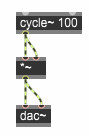
\includegraphics{img/pd_square.png}
		\caption{The square function in pure data, using a 100Hz sine as a test signal. What do you hear?}
		\label{fig:squarePd}
	\end{center}
\end{figure}



And we can simply plot what happened if we apply the function before also trying to understand analytically:


\begin{figure}[H]
	\begin{center}
		\includegraphics[width = 14cm]{img/sinSquared.png}
		\caption{Applying the square function to an input sine wave.}
		\label{fig:sinSquared}
	\end{center}
\end{figure}


Weird, the input seems to double in frequency (did you hear that?). Let's try to understand what's happening.\

So we calculate what happens if we send a cosine through this function, so let's take:

\begin{equation}
x = cos(\omega)
\end{equation}
wit arbitrary $\omega$. We can just ignore $\omega$ here for a while. Usually, there should be some indexing variable in the cosine function if we want to describe an oscillator that moves over time, but let's also skip that.\\
So applying our square function we of course get:
\begin{equation}
y = cos(\omega)^2
\end{equation}
This again results in:
\begin{equation}
y = cos(\omega) \cdot cos(\omega)
\end{equation}
So far so trivial. Note that a multiplication of two oscillators is called \textit{Amplitude Modulation} (actually, in this case we encounter ``Ring Modulation'', but let's ignore that also), and we know things about Amplitude modulation, namely:\

\fbox{
  \parbox{\textwidth}{
  When multiplying two oscillators, we get sum and difference of the two input frequencies. (And the whole output is attenuated by 6dB)
  }}
The above statement in equation form:
\begin{equation}
	cos(a)\cdot cos(b) = \frac{cos(a+b) + cos(a-b)}{2}
\end{equation}

We could also have looked up this \textit{trigonometric identity}.
This means for our experiment with our cosine squared:

\begin{equation}
y = \frac{cos(\omega+\omega) + cos(\omega-\omega)}{2}
\end{equation}
So:
\begin{equation}
y = \frac{cos(2 \cdot \omega) + cos(0)}{2} = \frac{cos(2 \cdot \omega )}{2}+\frac{1}{2}
\end{equation}

We arrive at the same result!
But is this true for every input? That would mean we just built a frequency shifter, did we? No. Waveshaping is much more complicated.\\

\begin{mdframed}[backgroundcolor=black!10,rightline=false,leftline=false]

This is immediately obvious when we try to do the same with two oscillators:
\begin{equation}
x = cos(\omega_1)+cos(\omega_2)
\end{equation}
then
\begin{equation}
y = (cos(\omega_1)+cos(\omega_2) ) ^2
\end{equation}
\begin{equation}
y = cos(\omega_1)^2+cos(\omega_2)^2+2\cdot cos(\omega_1) \cdot cos(\omega_2)
\end{equation}

And finally:
\begin{equation}
	y = \frac{cos(2 \cdot \omega_1)}{2} + \frac{1}{2} + \frac{cos(2 \cdot \omega_2)}{2} +\frac{1}{2} + 2 \cdot (\frac{cos(\omega_1+\omega_2) + cos(\omega_1-\omega_2)}{2})
\end{equation}

% \textbf{The point here is not to know this result by heart}, the point merely is that it's getting pretty complex.

\end{mdframed}

\subsection{How can waveshaping be implemented?} % (fold)
\label{sub:how_can_waveshaping_be_implemented_}


% subsection how_can_waveshaping_be_implemented_ (end)
Take a look at figure \ref{fig:tableVsCPU}. What do you think is happening?
On the left side, we see waveshaping as we did it above, using a mathematical function, in this case the tangens hyperbolicus, to distort our signal. On the right side, we see a table that contains the authors desperate attempt to draw the same function with the mouse. The results are theoretically equivalent (if the function in the table was correct), but what are the advantages and disadvantages of the two approaches?
Also, be sure to understand what the addition of 1 and the multiplication with 50 does on the right side. Hint: the array has 100 points.

\begin{figure}[H]
	\begin{center}
		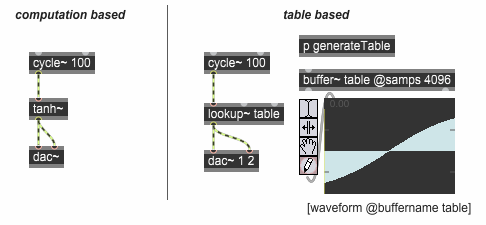
\includegraphics[width = 14cm]{tableVsCPU.png}
		\caption{Left: using a mathematical function to calculate the output. Right: using a table to look up the output.}
		\label{fig:tableVsCPU}
	\end{center}
\end{figure}





\subsection{How is Waveshaping related to other techniques?}
\subsubsection{Sampling}
If we take a look at figure \ref{fig:RamFilePlayback}, we see that we play a sound file by accessing a buffer (wavetable) using an index, an oscillator. This is effectively the same setup as we would build for distorting an input sound. Also take a look at figure \ref{fig:identity}, which showing us that waveshaping and wavetable synthesis are identical.

\begin{figure}[H]
	\centering
	\includegraphics[width=11cm]{identityWaveshaping.png}
	\caption[farnell waveshaping identity]
	{Picture taken from \cite{farnell_designing_2010}, showing the identity of waveshaping and wavetable synthesis}
	\label{fig:identity}
\end{figure}



\subsubsection{Modulation}
While we will talk about modulation in a separate chapter, let's loosely define amplitude modulation (AM) as the multiplication of two oscillators and frequency modulation (FM) as varying the frequency of an oscillator using another oscillator.\
So, as we have also seen above, AM looks like this:
\begin{equation}
	y = sin(a)\cdot sin(b)
\end{equation}

and FM looks like this:

\begin{equation}
	y = sin(sin(a))
\end{equation}

in practice, the a and b terms are a bit more complicated, but we will look at this later. That certain cases of AM are identical to waveshaping has been shown above, think about the square function again.
This of course does not mean that waveshaping can do everything AM can do and it does not mean that AM can achieve everything that waveshaping can. This should just show that we can understand the techniques from the perspective of another.\
What about FM? Well if our lookup function we use for waveshaping is a sine wave, we arrive at the exact same equation as how we defined FM above. Again, practically speaking, the results we get with these two techniques are very different, but we can see the connections.


\subsection{Why is Waveshaping useful?}
The output spectrum is dependent on the input amplitude. This makes it easy to create complex evolving spectra.

\subsection{What are the problems with waveshaping?}

Waveshaping adds overtones. When we build a waveshaper, we have to be aware of aliasing. Take a look at figures ~\ref{fig:clipped1} and ~\ref{fig:clipped2}. Sinewaves have been amplified and clipped here.

\begin{figure}[h!]
	\centering
	\includegraphics[width=11cm]{clippedSine.png}
	\caption[clipped sine wave]
	{A sine wave was generated and clipped. Clipping is a form of waveshaping which adds many overtones. Note how high frequencies fold back into the lower parts of the spectrum because they exceed the Nyquist-rate.}
	\label{fig:clipped1}
\end{figure}

\begin{figure}[h!]
	\centering
	\includegraphics[width=11cm]{clippedSine2.png}
	\caption[clipped sine wave 2]
	{Again, a sine wave, this time with a higher frequency to begin with. Extreme clipping has been applied by boosting the input amplitude. The aliased overtones are all over the place, even below the input frequency.}
	\label{fig:clipped2}
\end{figure}

In Max we could achieve this like in figure \ref{fig:pdClipping}.

\begin{figure}[H]
	\begin{center}
		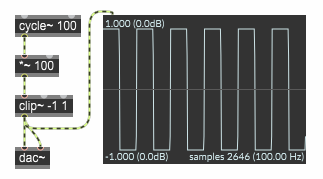
\includegraphics{img/pdSineClipping.png}
		\caption{Clipping an amplified sine wave in Max}
		\label{fig:pdClipping}
	\end{center}
\end{figure}

What does the output look like? Let's not only look at the spectra but also at the time signal:


\begin{figure}[H]
	\begin{center}
		\includegraphics[width = 14cm]{sineClipTime.png}
		\caption{An amplified and clipped sine wave in the time domain.}
		\label{fig:timeClip}
	\end{center}
\end{figure}

We see that we can arrive at a square-wave like result, but this square-wave is not anti-aliased.\\

The problem of aliasing in waveshaping is usually treated by over-sampling. This does not solve the problem but lessens it significantly resulting in cleaner, arguably better sound. Oversampling means that, if we work at a sample-rate of 44.1kHz, the input is up-sampled, essentially interpolated, to be at a sample-rate of 88.2kHz. Then the waveshaping is applied, leaving room for high frequencies up to 44.1kHz. Using a lowpass filter, high frequencies over 22.1kHz are then attenuated as much as possible, in order to be able to down-sample again to reach our initial sample-rate of 44.1kHz. \\
To state it more simple: Waveshaping is usually encapsulated in a process that runs at higher sampling rates in order to lessen aliasing.


% Wieso ist waveshaping praktisch? Amplitudenabhängigkeit d. spectrums.
% Wieso ist waveshaping verwandt mit modulation, sowohl FM, PM als auch AM? Am: siehe \(x^2\). FM: siehe \(f(x)=cos(x)\). Auch kann letztendlich eine transferkuntion in cos/sin bestandteile zerlegt werden um zu einer menge an frequenzmodulationen anzukommen, bzw kann der wavetable als polynom angenähert(o. Taylor entwicklung) werden um bei AM anzukommen.



\section{Sampler}
In pure data (but also in general) we can choose to play a sound from RAM or more or less\footnote{the data played from disk needs to be cached also} directly from the hard disk. Both Approaches have their different use-cases.\\


\video{In video, we need to make the same decision essentially. We can choose to buffer as much as we can on the VRAM of the graphics card or rather play from disk. Also different codecs specialize on balancing the load differently. The HAP codec for example tries to only push as much of the load to the hard disk and as little as possible to the CPU (which is decoding the video for playback). In times of SSDs this is a very good (and scalable) method to push a lot of data to playback in realtime.}
\textit{Work in progress.}

\begin{figure}[H]
	\begin{center}
		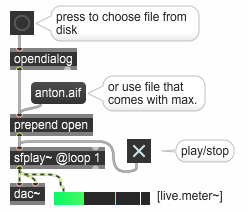
\includegraphics{img/sampler.png}
		\caption{Playback an audio file from disk.}
		\label{fig:simpleSampler}
	\end{center}
\end{figure}

% \begin{figure}[H]
% 	\begin{center}
% 		\includegraphics[scale = 0.5]{img/soundFileToRam2.png}
% 		\caption{sound in Ram}
% 		\label{fig:soundRam}
% 	\end{center}
% \end{figure}


\begin{figure}[H]
	\begin{center}
		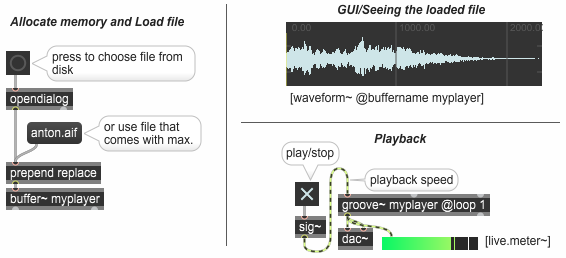
\includegraphics{img/RamFilePlayback.png}
		\caption{Audio file playback from RAM.}
		\label{fig:RamFilePlayback}
	\end{center}
\end{figure}



\begin{figure}[H]
	\begin{center}
		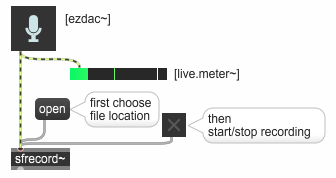
\includegraphics{writingAudio.png}
		\caption{writing Audio to disk}
		\label{fig:writing}
	\end{center}
\end{figure}

\bgInfo{
\subsection{Granular Sampling}
In figure \ref{fig:granular} you see the basic structure of granular sampling. Granular sampling allows us for example to playback a file slower without lowering the pitch. It is one of the methods to make speed and ppitch independent from each other during playback. Other methods also include FFT based approaches.

\begin{figure}[H]
	\begin{center}
		\includegraphics[width=\textwidth]{img/grain2.png}
		\caption {The patcher \href{./patchers/01\_waveshaping/granular.pd}{\texttt{patchers/01\_waveshaping/granular.pd}}, a simplified version of granular sampling}
		\label{fig:granular}
	\end{center}
\end{figure}
}


\section{Key Points}

\begin{itemize}
	\item When do we sampling from RAM when from disk?
	\item what are the problems with waveshaping?
	\item Make sure you understand that waveshaping can produce overtones.
	\item Make sure if you see a (simple) mathematical expression you can decide if it is non-linear or not.
	\item Make sure you recognize waveshaping in Max if you see it (e.g. figure \ref{fig:squarePd} )
\end{itemize}


% \section{Hausübung}
% \subsection{Testmodul}

% baue ein audio Testmodul mit folgener spezifikation:\\
% \begin{itemize}
% 	\item Ein audio output
% 	\item verschiedene klangquellen wählbar:
% 		\begin{enumerate}
% 			\item White Noise
% 			\item Sinus (freq. einstellbar)
% 			\item soundfile (file wählbar)
% 		\end{enumerate}
% 	\item GUI
% 	\item verfügbar(in eurem pfad, und jederzeit abrufbar als abstraction)
% 	\item output pegel sichtbar (level meter)
% \end{itemize}


% \begin{figure}[H]
% 	\begin{center}
% 		\includegraphics[scale = 1]{img/audioTester.png}
% 		\caption{audioTester.pd, zu bauen als Hausübung}
% 		\label{fig:audiotester}
% 	\end{center}
% \end{figure}
